%TODO 
%Bilder zitieren

\renewcommand{\theauthor}{Matthias Franz}
\chapter{Datenbank}
\label{sec:datenbank}
In diesem Kapitel geht es um die Datenbank welche in dieser Arbeit erstellt worden ist. Es geht um den Aufbau der Datenbank, deren Funktion und wie diese mit den anderen Teilen des Projektes zusammenarbeitet.

\section{Funktion der Datenbank}
\label{sec:funktionDatenbank}
Die Datenbank speichert Benutzerdaten und Kalender der Benutzer. Die Daten dieser Datenbank bilden alle für dieses Projekt relevanten Teile einer iCal-Datei ab. Es werden nicht alle möglichen Eigenschaften einer iCal-Datei benötigt, da die Daten welche gespeichert werden ausreichen, um einen typischen Kalender welcher in Unternehmen verwendet wird abgebildet. Die Datenbank ermöglicht es, dass mehrere Benutzer mehrere Kalender haben und mehrere Benutzer auch die gleichen Kalender haben können. Benutzer sind in der Lage Kalender mit Terminen, To-Do Elementen und Alarmen zu speichern, weiters ermöglicht die Datenbank es die Zeitzone des Kalenders zu ändern.
\\
Die Daten werden dann vom Parser genommen und in eine funktionierende .ics-Datei umgewandelt. 

\section{Aufbau der Datenbank}
\label{sec:aufbauDatenbank}
Die Datenbank ist relationale Datenbank MSSQL-Datenbank, das ER-Diagramm welches in Abbildung \ref{fig:erDiagramm} zu sehen ist wurde mit der Krähenfuß- oder auch Martinnotation abgebildet. 
\\
Ein ER-Diagramm besteht aus Entitäten und Relationen, eine Entität ist eine Tabelle und eine Relation ist eine Verbindung zweier Entitäten. Eine Relation hat immer zwei Kardinalitäten, eine Kardinalität gibt die maximal möglich Anzahl an Instanzen auf welche sich eine Entität referenzieren kann. In der Krähenfußnotation gibt es sechs verschiedene Kardinalitäten. Da auf jeder der beiden Seiten einer Relation eine Kardinalität ist, gibt es viele verschiedene Kombinationen. Alle möglichen Kardinalitäten werden in Abbildung \ref{fig:kardinalitaeten} gezeigt.
\begin{figure}[H]
	\centering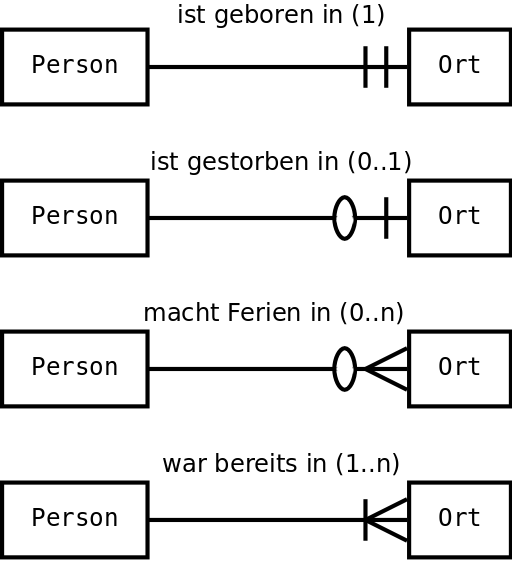
\includegraphics[scale=0.7]
	{Datenbank_Kardinalitaeten.png}
    \caption{Kardinalitäten}
    \label{fig:kardinalitaeten}
\end{figure}
Im ER-Diagramm von Abbildung \ref{fig:erDiagramm} werden Primary-Keys fett und Foreign Keys kursiv dargestellt.

\begin{figure}[H]
	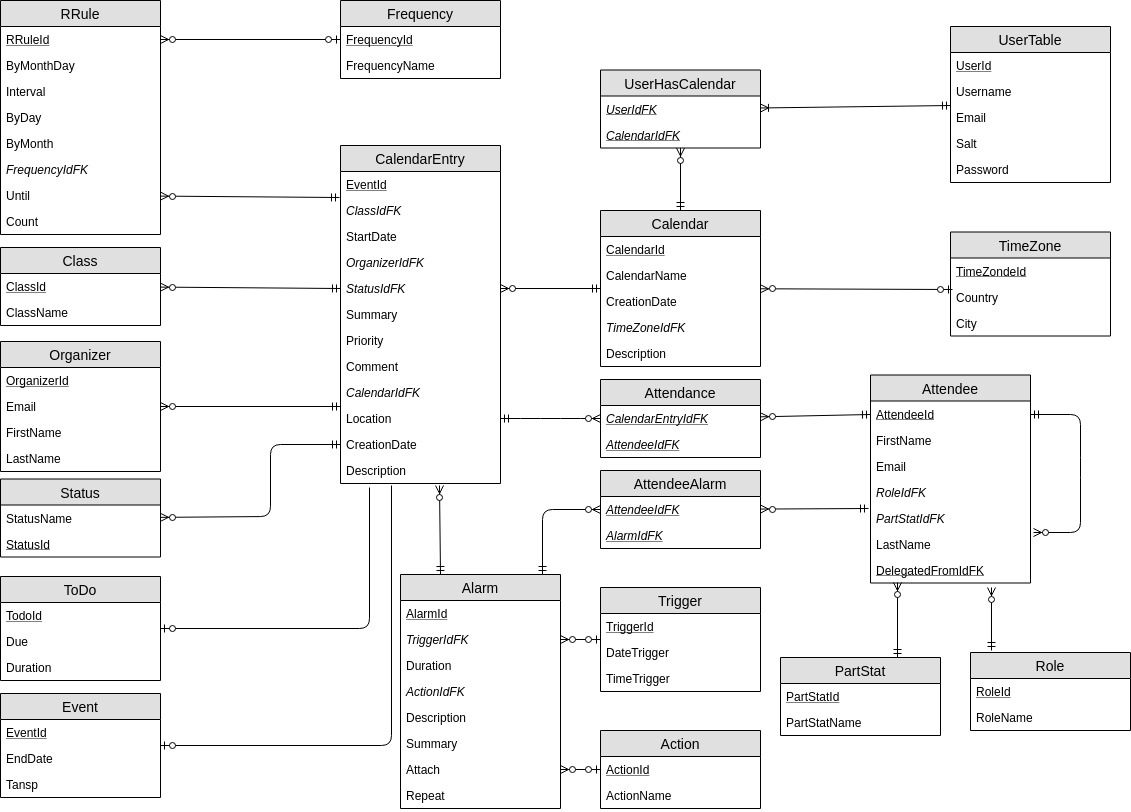
\includegraphics[angle=270,origin=c,width=\textwidth]{Datenbank_ER-Diagramm.jpg}
    \caption{ER-Diagramm}
    \label{fig:erDiagramm}
\end{figure}

\subsubsection*{Benutzer und Kalender}
\label{ref:benutzerKalender}
In der UserTable-Tabelle werden Benutzerdaten gespeichert, jeder Benutzer bekommt eine einmalide Id zugewiesen, die UserId. Weiters wird von jeden Benutzer ein Benutzername, eine Email und ein Passwort gespeichert. Genaueres zum UserTable ist im Kapitel \ref{sec:UserDB}. Da ein Benutzer mehrere Kalender haben kann und ein Kalender auch zu mehreren Benutzern gehört, gibt es die Tabelle UserHasCalendar, welche dazu dient, festzuhalten welcher Kalender zu welchen Benutzern gehört. Dies wird erreicht indem der Primary-Key der UserTable-Tabelle und der Calender-Tabelle zusammen als Primary-Key in der UserHasCalender-Tabelle genommen werden.Wie dies im ER-Diagramm aussieht sieht man in Abbildung \ref{fig:userCalender}.\\
Die Calender-Tabelle speichert Informationen zu einem Kalender welche dann im Parser in die iCal-Datei gegeben werden.
\begin{figure}[H]
	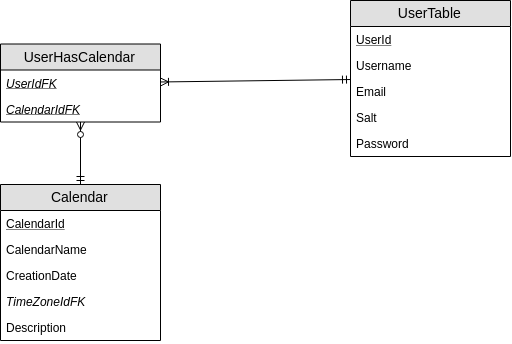
\includegraphics[width=\textwidth]{Datenbank_UserCalendar.png}
    \caption{Relation zwischen Benutzer und Kalender}
    \label{fig:userCalender}
\end{figure}

\subsubsection*{Kalender und Zeitzonen}
\label{ref:kalenderZeitzonen}
Da dieses Projekt für ein Unternehmen gemacht wurde, welches mit Internationalen Kunden tätig ist, ist es wichtig, dass Kalender in verschiedenen Zeitzonen seien können. Deswegen wurde eine eigene Tabelle mit Zeitzonen angefertigt, damit das hinzufügen von einer Zeitzone in einen Kalender einfacher wird. Die TimeZone-Tabelle welche Zeitzonen abbildet besteht aus einer einmaligen Id und dem Land und der Stadt der Zeitzone, da im iCal-Format Zeitzonen so abgebildet werden. 
\begin{figure}[H]
	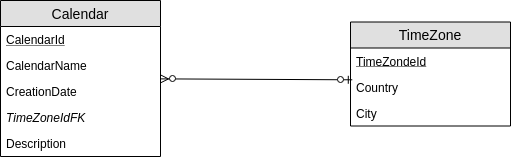
\includegraphics[width=\textwidth]{Datenbank_CalendarTimezone.png}
    \caption{Relation zwischen Kalender und Zeitzone}
    \label{fig:timezoneCalender}
\end{figure}

\subsubsection*{Kalendereinträge}
\label{ref:kalenderEintraege}
Ein Kalender besteht aus mehreren Kalendereinträgen, ein Kalenderbeitrag ist zum Beispiel ein Termin oder ein To-Do Element. Termine werden in der Event-Tabelle und To-Dos in der ToDo-Tabelle abgebildet. Da diese beiden Objekte viele ähnliche Attribute haben aber dennoch einige Attribute besitzen welche die andere Tabelle nicht benötigt, sind sie beide mit der gleichen Supertabelle über eine is-a Relation verbunden. Is-a bedeutet, dass beide Tabellen alle Attribute der CalendarEntry-Tabelle zusätzlich zu ihren eigenen Attributen besitzen.
\begin{figure}[H]
	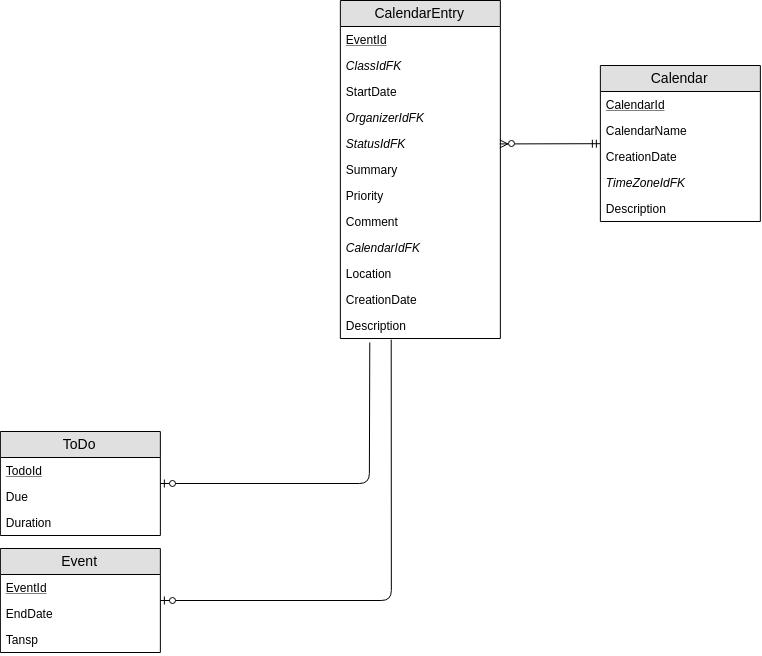
\includegraphics[width=\textwidth]{Datenbank_CalenderEntries.png}
    \caption{Kalendereinträge}
    \label{fig:calendarEntries}
\end{figure}


	